\vspace{-0.3cm}
\section{Evaluation}
\vspace{-0.2cm}

We extensively evaluated \sys against various state-of-the-art methods and systems. Our results show that:
\begin{enumerate}[label=(\arabic*), leftmargin=0.5cm, noitemsep,topsep=0pt]
\item \sys achieves orders of magnitude speedup over T10 and Ladder in LLM inference (\S\ref{sec:eval:e2e});
\item \sys{}'s 
\gemm and \gemv perform and scale strongly over the state-of-the-art (\S\ref{sec:eval:meshgemm});
\item \sys's shift-based KV cache management enables over 360-385$\times$ more token capacity (\S\ref{sec:eval:kvcache});
\item \sys on Cerebras WSE-2 achieves 10-20$\times$ e2e speedup compared to the optimal performance of SGLang on A100 GPUs-cluster, and about 30-40$\times$ speedup compared to a single A100 GPU. \sys also achieves approximately 2.5$\times$ better energy efficiency (\S\ref{sec:eval:e2e},\S\ref{sec:eval:gpu}).
\end{enumerate}

\mypar{Experiment setup}
We evaluate \sys on a server with Cerebras WSE-2. WSE-2 has 850,000 Cores, each with a Compute Engine (CE) operating at a maximum of 1.1 GHz. Each clock cycle can fetch two 32-bit operands from SRAM, perform a multiply-accumulate operation, and then write back to SRAM. Each core also has a fabric router that can send or receive 32-bit messages from neighbouring cores with a single clock cycle. Additionally, each core contains 48KB of SRAM, with the chip totalling 40GB of aggregated SRAM~\cite{wse}.

We compare \sys with two DNN compilers: (i)T10\cite{t10}, the state-of-the-art compiler for AI accelerators with inter-core connections and distributed on-chip memory, and (ii)Ladder\cite{ladder}, the state-of-the-art compiler for shared memory architectures. For T10, we implemented it on WSE-2, treating each core as part of a distributed memory system interconnected by a crossbar, despite the actual mesh topology. T10 maps data to core IDs and fetches data from local SRAM as required. For Ladder, we treated the distributed memory architecture of the chip, interconnected by mesh, as unified memory, requiring collective communication over the NoC to access data.

We use the Nvidia A100 for GPU comparison experiments, which shares the same 7nm process as the WSE-2 for fairness. The experiments utilize up to 16 GPUs across two nodes (2$\times$8 configuration). Within a single node, the eight A100 GPUs are interconnected via NVLink, while inter-node communication is handled through a high-performance InfiniBand (IB) network. We use SGLang\cite{sglang}, one of the highest-performing LLM inference systems for GPU-based experiments.

\mypar{Experiment metric} To evaluate the maximum per-request throughput performance of LLM inference systems on different hardware, we define Throughput per Request (TPR) as a key metric. TPR is derived from the more widely used Time per Output Token (TPOT), with $\text{TPR} = \frac{1}{\text{TPOT}}$.

\mypar{LLM models}
Our evaluation includes various representative LLMs of different sizes and architectures. Specifically, LLaMA3-8B and LLaMA2-13B are widely used open-source LLMs, with LLaMA3 using group-query attention instead of multi-head attention to reduce KV cache usage. For LLaMA2-13B, we modified the model to remove the 4K context length limitation to evaluate system performance across different input and output lengths. Additionally, due to the tensor parallelism constraints, the number of attention heads of a model must be divisible by the number of GPUs used. We did not conduct the multi-GPU experiment of LLaMA-2 on a 16-GPU cluster. CodeLLaMA-34B is a specialized LLM for coding tasks, while QWen2-72B, another popular LLM, is renowned for its high model quality.

\vspace{-0.2cm}
\subsection{LLM inference} \label{sec:eval:e2e}

We first report the end-to-end performance of \sys compared to T10 and Ladder on WSE-2 and SGLang on the A100 GPU cluster. Then we further analyze the performance to provide deeper insights by breaking down the execution into prefill and decode phases.

\begin{table}[t]
  \centering
  \resizebox{\linewidth}{!}{
    \begin{tabular}{l|cc|cccc}
\hline
\multicolumn{1}{c|}{\multirow{2}{*}{Model}} & \multicolumn{2}{c|}{\multirow{2}{*}{Device}} & \multicolumn{4}{c}{Input/Output Seqence Length} \\ \cline{4-7} 
\multicolumn{1}{c|}{} & \multicolumn{2}{c|}{} & \multicolumn{1}{c|}{2048/128} & \multicolumn{1}{c|}{4096/128} & \multicolumn{1}{c|}{2048/2048} & 4096/4096 \\ \hline
\multirow{6}{*}{LLaMA3-8B} & \multicolumn{1}{c|}{\multirow{3}{*}{WSE-2}} & \sys & \multicolumn{1}{c|}{764.4} & \multicolumn{1}{c|}{604.4} & \multicolumn{1}{c|}{2370.3} & 2459.0 \\
 & \multicolumn{1}{c|}{} & T10 & \multicolumn{1}{c|}{4.6} & \multicolumn{1}{c|}{4.5} & \multicolumn{1}{c|}{58.3} & 94.6 \\
 & \multicolumn{1}{c|}{} & Ladder & \multicolumn{1}{c|}{1.2} & \multicolumn{1}{c|}{1.1} & \multicolumn{1}{c|}{7.4} & 8.7 \\ \cline{2-7} 
 & \multicolumn{1}{c|}{\multirow{3}{*}{\begin{tabular}[c]{@{}c@{}}A100 GPU\\ (SGLang)\end{tabular}}} & 1 & \multicolumn{1}{c|}{34.8} & \multicolumn{1}{c|}{31.1} & \multicolumn{1}{c|}{36.5} & 78.4 \\
 & \multicolumn{1}{c|}{} & 8 & \multicolumn{1}{c|}{117.2} & \multicolumn{1}{c|}{109.0} & \multicolumn{1}{c|}{128.4} & 256.1 \\
 & \multicolumn{1}{c|}{} & 2$\times$8 & \multicolumn{1}{c|}{73.7} & \multicolumn{1}{c|}{70.2} & \multicolumn{1}{c|}{79.3} & 162.5 \\ \hline
\multirow{5}{*}{LLaMA2-13B} & \multicolumn{1}{c|}{\multirow{3}{*}{WSE-2}} & \sys & \multicolumn{1}{c|}{473.9} & \multicolumn{1}{c|}{414} & \multicolumn{1}{c|}{1690.3} & 1826.0 \\
 & \multicolumn{1}{c|}{} & T10 & \multicolumn{1}{c|}{2.6} & \multicolumn{1}{c|}{2.5} & \multicolumn{1}{c|}{35.0} & 58.3 \\
 & \multicolumn{1}{c|}{} & Ladder & \multicolumn{1}{c|}{0.7} & \multicolumn{1}{c|}{0.7} & \multicolumn{1}{c|}{4.9} & 6.1 \\ \cline{2-7} 
 & \multicolumn{1}{c|}{\multirow{2}{*}{\begin{tabular}[c]{@{}c@{}}A100 GPU\\ (SGLang)\tablefootnote{\label{missing_16GPU}No 2$\times$8 GPUs, due to model architecture and tensor parallelism.}\end{tabular}}} & 1 & \multicolumn{1}{c|}{20.4} & \multicolumn{1}{c|}{17.1} & \multicolumn{1}{c|}{21.1} & 47.9 \\
 & \multicolumn{1}{c|}{} & 8 & \multicolumn{1}{c|}{79.6} & \multicolumn{1}{c|}{70.5} & \multicolumn{1}{c|}{86.9} & 172.4 \\ \hline
\end{tabular}%
    }
  \caption{End-to-end LLM inference TPR}
  \label{tab:e2e_table}%
\end{table}%

\mypar{End-to-end throughput} Table~\ref{tab:e2e_table} shows the inference TPR of LLaMA3-8B and LLaMA2-13B on WSE-2 and A100 with different input and output sequence lengths. Here, the end-to-end throughput is calculated as the total number of tokens generated during the decode phase divided by the total time spent in the prefill and decode phases. \sys uses core configurations optimized for the best performance with each model.
In LLaMA3-8B, we use 660$\times$660 cores for prefill and 360$\times$360 for decode.
In LLaMA2-13B, we use 750$\times$750 cores for prefill and 375$\times$375 for decode.
CodeLLaMA-34B and QWen2-72B are not included due to the memory constraint of a single WSE-2 chip.

Compared to T10, \sys achieves 160$\times$ speedup on average, up to 180$\times$, for short sequence generation tasks such as 4096 and 2048 input context lengths with 128 tokens output. For longer tasks, with input context lengths of 4096 and 2048 tokens and output lengths of 4096 and 2048 tokens, \sys achieves 36$\times$ on average and up to 48$\times$. Although T10 designs the compute-shift model that considers the memory constraints (M) and routing resource limits (R) of a PLMR device, it does not account for the cores interconnected by a mesh NoC. Thus, failing to address varying hop distances (L) and scale to millions of cores (P), highlighting the need for new system designs in massive-scale NUMA architectures.

Compared to Ladder, \sys achieves 625$\times$ speedup on average, up 677$\times$, for short sequence generation tasks such as 4096 and 2048 input context lengths with 128 tokens output. For longer sequence generation tasks, with input context lengths of 4096 and 2048 tokens and output lengths of 4096 and 2048 tokens, \sys achieves 312$\times$ on average and up to 342$\times$. That is because Ladder is designed for shared memory architecture and does not consider the characteristics of the PLMR device, resulting in failure in partitioning LLMs across millions of cores (P), incurring costly long-range NoC communication (L), failure in handling local memory constraints (M) and limited routing resources (R).

\begin{table}[t]
\centering
\resizebox{\linewidth}{!}{
\begin{tabular}{c|c|ccclccc}
\cline{1-5} \cline{7-9}
\multirow{2}{*}{Model} & \multirow{2}{*}{Methods} & \multicolumn{3}{c}{WSE-2 Cores} &  & \multicolumn{3}{c}{\# A100 GPUs (SGLang)} \\ \cline{3-5} \cline{7-9} 
 &  & \multicolumn{1}{c|}{480$\times$480} & \multicolumn{1}{c|}{600$\times$600} & 720$\times$720 &  & \multicolumn{1}{c|}{1} & \multicolumn{1}{c|}{8} & 2$\times$8 \\ \cline{1-5} \cline{7-9} 
\multirow{3}{*}{LLaMA3-8B} & \sys & \multicolumn{1}{c|}{20320.6} & \multicolumn{1}{c|}{25037.2} & 27686.5 &  & \multicolumn{1}{c|}{\multirow{3}{*}{13988.3}} & \multicolumn{1}{c|}{\multirow{3}{*}{17361.6}} & \multirow{3}{*}{13994.2} \\
 & T10 & \multicolumn{1}{c|}{175.0} & \multicolumn{1}{c|}{156.6} & 132.8 &  & \multicolumn{1}{c|}{} & \multicolumn{1}{c|}{} &  \\
 & Ladder & \multicolumn{1}{c|}{61.8} & \multicolumn{1}{c|}{42.3} & 31.3 &  & \multicolumn{1}{c|}{} & \multicolumn{1}{c|}{} &  \\ \cline{1-5} \cline{7-9} 
\multirow{3}{*}{LLaMA2-13B} & \sys & \multicolumn{1}{c|}{13685.1} & \multicolumn{1}{c|}{16854.2} & 17498.3 &  & \multicolumn{1}{c|}{\multirow{3}{*}{7805.1}} & \multicolumn{1}{c|}{\multirow{3}{*}{12287.1}} & \multirow{3}{*}{/\textsuperscript{\ref{missing_16GPU}}} \\
 & T10 & \multicolumn{1}{c|}{121.3} & \multicolumn{1}{c|}{100.6} & 81.3 &  & \multicolumn{1}{c|}{} & \multicolumn{1}{c|}{} &  \\
 & Ladder & \multicolumn{1}{c|}{47.3} & \multicolumn{1}{c|}{33.1} & 24.2 &  & \multicolumn{1}{c|}{} & \multicolumn{1}{c|}{} &  \\ \cline{1-5} \cline{7-9} 
\multirow{3}{*}{CodeLLaMA-34B} & \sys & \multicolumn{1}{c|}{5471.4} & \multicolumn{1}{c|}{7540.1} & 8526 &  & \multicolumn{1}{c|}{\multirow{3}{*}{5382.5}} & \multicolumn{1}{c|}{\multirow{3}{*}{7155.5}} & \multirow{3}{*}{6409.2} \\
 & T10 & \multicolumn{1}{c|}{49.1} & \multicolumn{1}{c|}{46.8} & 41.2 &  & \multicolumn{1}{c|}{} & \multicolumn{1}{c|}{} &  \\
 & Ladder & \multicolumn{1}{c|}{30.1} & \multicolumn{1}{c|}{23.1} & 17.7 &  & \multicolumn{1}{c|}{} & \multicolumn{1}{c|}{} &  \\ \cline{1-5} \cline{7-9} 
\multirow{3}{*}{QWen2-72B} & \sys & \multicolumn{1}{c|}{2785.2} & \multicolumn{1}{c|}{3775.5} & 4421.6 &  & \multicolumn{1}{c|}{\multirow{3}{*}{1677.3}} & \multicolumn{1}{c|}{\multirow{3}{*}{3803.8}} & \multirow{3}{*}{3750.5} \\
 & T10 & \multicolumn{1}{c|}{24.9} & \multicolumn{1}{c|}{23.5} & 21.5 &  & \multicolumn{1}{c|}{} & \multicolumn{1}{c|}{} &  \\
 & Ladder & \multicolumn{1}{c|}{16.8} & \multicolumn{1}{c|}{12.8} & 10.1 &  & \multicolumn{1}{c|}{} & \multicolumn{1}{c|}{} &  \\ \cline{1-5} \cline{7-9} 
\end{tabular}%
}
  \caption{Prefill Throughput per Request (TPR)}
  \vspace{-0.2cm}
\label{tab:prefill_throughput}
\end{table}%

\mypar{Prefill throughput} Table~\ref{tab:prefill_throughput} shows the prefill performance for an input sequence length of 4096, using core configurations from 480$\times$480 to 720$\times$720. For CodeLLaMA-34B and QWen2-72B, which exceed the memory capacity of WSE-2 and a single A100, we evaluate a subset of layers and scale the results proportionally due to their uniform layer structure.

\sys achieves significant speedups over T10 and Ladder by effectively addressing all PLMR properties, an average speedup of ~160$\times$ (up to 178$\times$) over T10 and ~270-450$\times$ over Ladder. As discussed in Section~\S\ref{sec:motivation}, GEMM is the primary bottleneck, and \gemm substantially enhances \sys's prefill performance, analyzed in detail in Section~\S\ref{sec:eval:meshgemm}.

Additionally, \sys scales throughput with increasing cores across all models. For instance, \sys achieves a 1.6$\times$ scaleup on QWen2-72B and a 1.4$\times$ scaleup on LLaMA3-8B when scaling from 480$\times$480 to 720$\times$720 cores. In contrast, T10 and Ladder fail to scale effectively, with throughput even declining as more cores are added. This is mainly because T10 and Ladder do not account for the spatial locality characteristic (L) of highly uniformly distributed memory, which can lead to frequent long-distance data reads across cores and increased communication overhead.

\begin{table}[t]
  \centering
  \resizebox{\linewidth}{!}{
    \begin{tabular}{c|c|ccclccc}
\cline{1-5} \cline{7-9}
\multirow{2}{*}{Model} & \multirow{2}{*}{Methods} & \multicolumn{3}{c}{WSE-2 Cores} &  & \multicolumn{3}{c}{\# A100 GPUs (SGLang)} \\ \cline{3-5} \cline{7-9} 
 &  & \multicolumn{1}{c|}{420$\times$420} & \multicolumn{1}{c|}{540$\times$540} & 660$\times$660 &  & \multicolumn{1}{c|}{1} & \multicolumn{1}{c|}{8} & 2$\times$8 \\ \cline{1-5} \cline{7-9} 
\multirow{3}{*}{LLaMA3-8B} & \sys & \multicolumn{1}{c|}{2699.9} & \multicolumn{1}{c|}{2501.5} & 2243.3 &  & \multicolumn{1}{c|}{\multirow{3}{*}{78.9}} & \multicolumn{1}{c|}{\multirow{3}{*}{260.4}} & \multirow{3}{*}{164.6} \\
 & T10 & \multicolumn{1}{c|}{418.3} & \multicolumn{1}{c|}{339.4} & 265.1 &  & \multicolumn{1}{c|}{} & \multicolumn{1}{c|}{} &  \\
 & Ladder & \multicolumn{1}{c|}{14.6} & \multicolumn{1}{c|}{13.1} & 11.4 &  & \multicolumn{1}{c|}{} & \multicolumn{1}{c|}{} &  \\ \cline{1-5} \cline{7-9} 
\multirow{3}{*}{LLaMA2-13B} & \sys & \multicolumn{1}{c|}{2039.2} & \multicolumn{1}{c|}{1899.4} & 1739.8 &  & \multicolumn{1}{c|}{\multirow{3}{*}{48.7}} & \multicolumn{1}{c|}{\multirow{3}{*}{175.8}} & \multirow{3}{*}{/\textsuperscript{\ref{missing_16GPU}}} \\
 & T10 & \multicolumn{1}{c|}{341.8} & \multicolumn{1}{c|}{270.8} & 233.7 &  & \multicolumn{1}{c|}{} & \multicolumn{1}{c|}{} &  \\
 & Ladder & \multicolumn{1}{c|}{11.0} & \multicolumn{1}{c|}{9.9} & 9.0 &  & \multicolumn{1}{c|}{} & \multicolumn{1}{c|}{} &  \\ \cline{1-5} \cline{7-9} 
\multirow{3}{*}{CodeLLaMA-34B} & \sys & \multicolumn{1}{c|}{1450.8} & \multicolumn{1}{c|}{1407.7} & 1359.2 &  & \multicolumn{1}{c|}{\multirow{3}{*}{26.1}} & \multicolumn{1}{c|}{\multirow{3}{*}{100.4}} & \multirow{3}{*}{84.5} \\
 & T10 & \multicolumn{1}{c|}{278.2} & \multicolumn{1}{c|}{222.4} & 193.1 &  & \multicolumn{1}{c|}{} & \multicolumn{1}{c|}{} &  \\
 & Ladder & \multicolumn{1}{c|}{6.1} & \multicolumn{1}{c|}{6.2} & 5.8 &  & \multicolumn{1}{c|}{} & \multicolumn{1}{c|}{} &  \\ \cline{1-5} \cline{7-9} 
\multirow{3}{*}{QWen2-72B} & \sys & \multicolumn{1}{c|}{839.7} & \multicolumn{1}{c|}{824.3} & 787.1 &  & \multicolumn{1}{c|}{\multirow{3}{*}{10.6}} & \multicolumn{1}{c|}{\multirow{3}{*}{51.2}} & \multirow{3}{*}{48.7} \\
 & T10 & \multicolumn{1}{c|}{168.5} & \multicolumn{1}{c|}{133.0} & 114.6 &  & \multicolumn{1}{c|}{} & \multicolumn{1}{c|}{} &  \\
 & Ladder & \multicolumn{1}{c|}{3.2} & \multicolumn{1}{c|}{3.3} & 3.4 &  & \multicolumn{1}{c|}{} & \multicolumn{1}{c|}{} &  \\ \cline{1-5} \cline{7-9} 
\end{tabular}%
    }
  \caption{Decode Throughput per Request (TPR)}
  \vspace{-0.2cm}
\label{tab:decode_throughput}
\end{table}%

\mypar{Decode throughput} Table~\ref{tab:decode_throughput} shows decode throughput for core configurations from 420$\times$420 to 660$\times$660. For CodeLLaMA-34B and QWen2-72B decode benchmark on WSE-2 and single A100, we evaluate a subset of layers and scale the results.

By addressing all PLMR properties, \sys achieves an average speedup of 5.7$\times$ (up to 6.5$\times$) over T10 and 217$\times$ (up to 260$\times$) over Ladder.

Compared to the 160$\times$ speedup \sys achieves over T10 during prefill, it offers only about a 6.5$\times$ speedup during decode. However, \sys maintains a consistent 200-500$\times$ advantage over Ladder in both prefill and decode stages. This is mainly because prefill involves dist-GEMM computations, which require each data element to traverse cores along the same row or column sequentially. In contrast, the dist-GEMV allreduce operation in decode only requires traversal across cores in the same row or column, without enforcing a strict access order. While T10’s compute-shift paradigm does not consider the spatial locality of cores on a mesh NoC, it still accounts for distributed memory, which allows performance gains when memory (communication) accesses are order-independent. In contrast, Ladder is entirely designed for a shared memory architecture, leading to severe communication overhead regardless of whether memory access order is required.

\mypar{Comparison with SGLang} As shown in Table~\ref{tab:e2e_table},\ref{tab:prefill_throughput} and \ref{tab:decode_throughput}, \sys demonstrates clear advantages over SGLang + A100 GPU clusters in prefill, decode tasks, and also the end-to-end performance across models ranging from 8B to 72B. More detailed comparisons with GPUs are discussed in Section~\S\ref{sec:eval:gpu}.

It is worth noting that T10 and Ladder fail to leverage the powerful hardware capabilities of the WSE-2 when compared to SGLang. For example, in prefill tasks and for Ladder in decode tasks, their performance is even worse than that of SGLang running on a single A100. This highlights that designing high-performance systems and algorithms on wafer-scale chips must carefully consider the PLMR model; otherwise, not only will the massive compute potential of the chip go underutilized, but performance may even degrade due to the highly uniform distributed memory resulting from the large-scale mesh NoC.

\vspace{-0.2cm}
\subsection{\gemm}\label{sec:eval:meshgemm}
\vspace{-0.2cm}

\begin{figure}
    \centering
    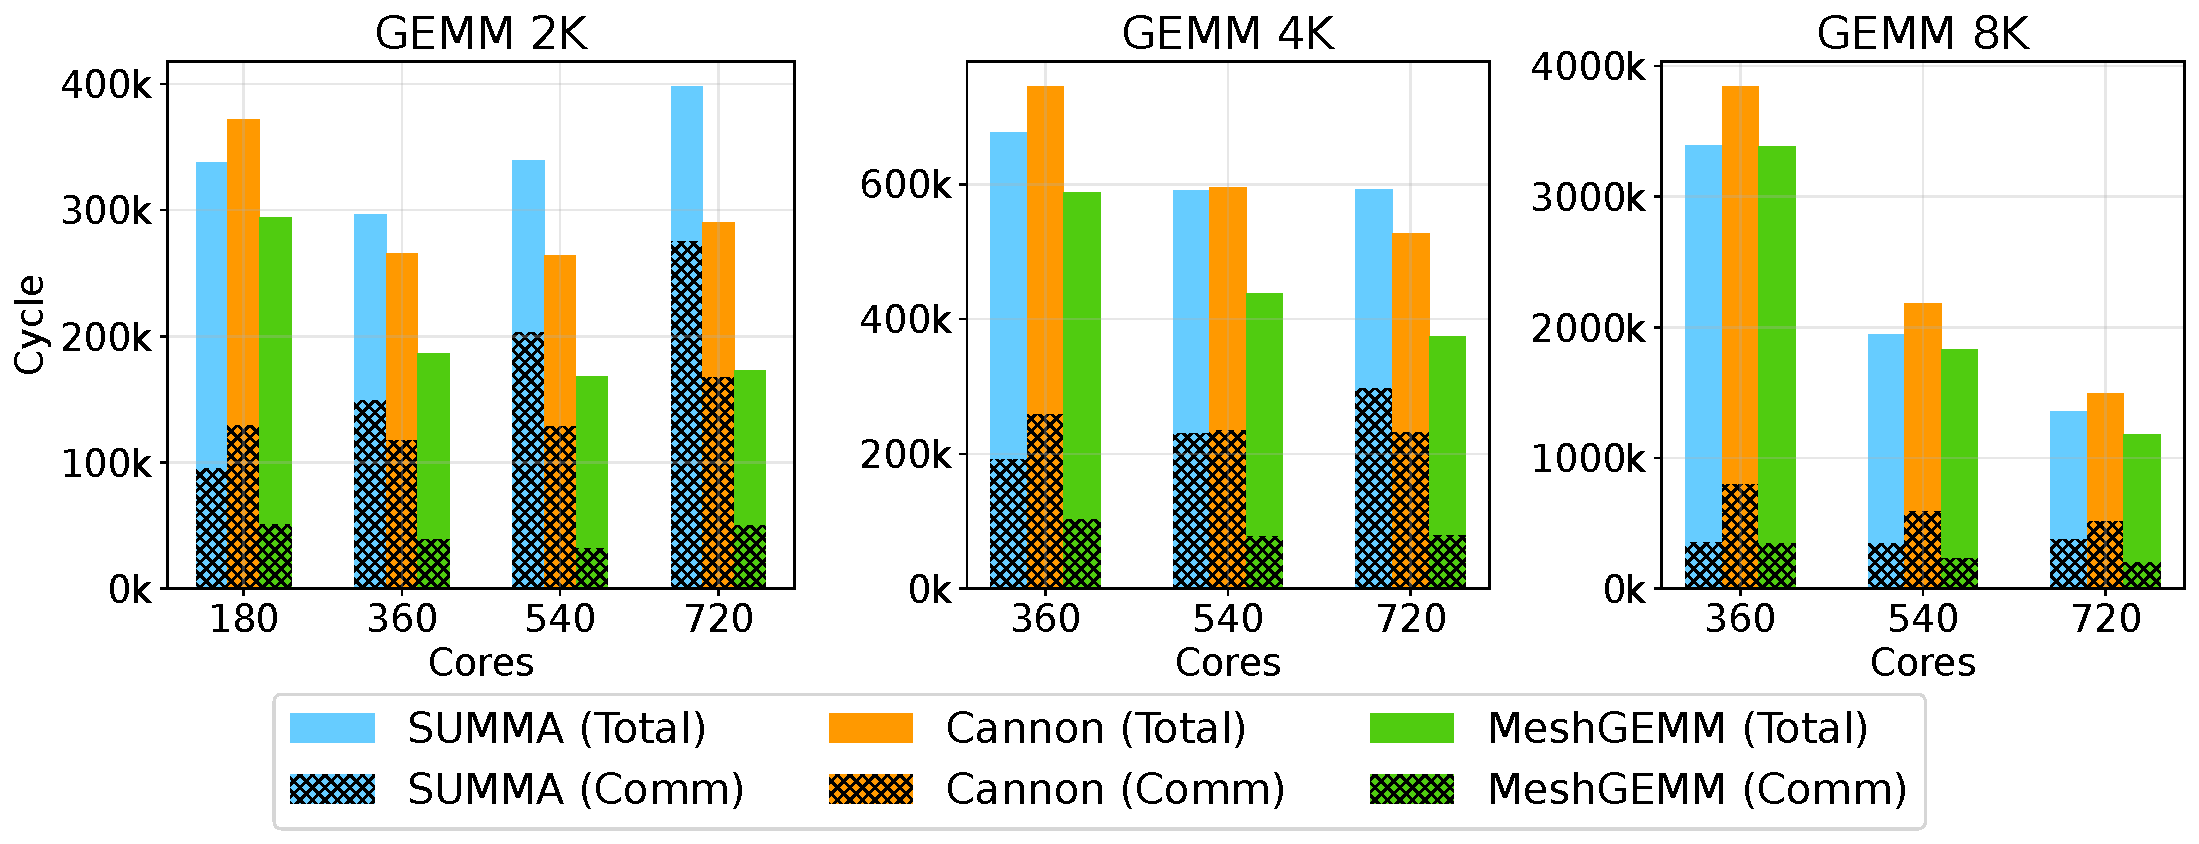
\includegraphics[width=1\linewidth]{imgs/gemm_micro_benchmark_combined.pdf}
    \caption{\gemm vs. SUMMA \& Cannon}
    \vspace{-0.5cm}
    \label{fig:eval:meshgemm}
\end{figure}

We compare \gemm with Cannon~\cite{cannon} and SUMMA~\cite{summa} on WSE-2 across different core scales and matrix sizes.

\mypar{Scaling core count} 
Figure~\ref{fig:eval:meshgemm} shows that across matrices of different sizes, \gemm can achieve the lowest latency than SUMMA and Cannon by scaling up the number of cores. Compared to the pipeline broadcast in SUMMA and head-to-tail transmission in Cannon, interleave transmission in \gemm can minimize per-step communication overhead and, as much as possible, overlap communication with computation during large-scale fine-grained parallel execution. It demonstrates stronger scalability, maintaining over 70\% computational efficiency even near the hardware limit. In contrast, SUMMA and Cannon exhibit poor scalability, with computational efficiency falling below 50\% with 720$\times$720 cores, primarily due to the communication overhead in SUMMA and Cannon, increasing with the parallelism scale.

Additionally, increasing the number of cores does not always bring performance gains, especially for small matrix GEMM tasks. For example, in GEMM 2K, when scaling from 360$\times$360 to 720$\times$720 cores, the end-to-end latency of SUMMA and Cannon increases instead of decreasing. This is because the per-core computation cost drops sublinearly as cores increase beyond a threshold (due to fixed overheads like function calls and logic checks). At the same time, communication overhead grows linearly, as seen from the shaded areas in Figure~\ref{fig:eval:meshgemm}, leading to worse overall performance. In contrast, \gemm only shows a slight communication overhead increase at 720$\times$720 cores and maintains stable end-to-end latency. This is because its interleave communication bounds the per-step communication cost to a constant, independent of core count (the total communication overhead grows only because the number of steps increases in all dist-GEMM algorithms). Thus, \gemm can achieve a better overlapping between communication and computation even under large-scale fine-grained parallelism (each core is only responsible for a small amount of data).

\mypar{Scaling matrix size} We also evaluate \gemm with larger matrix sizes, transforming GEMM into a more computationally intensive operation. At large scales, though the cost of communication becomes less significant, \gemm maintains its scalability and outperforms SUMMA and Cannon by a wide margin, reducing total cycles by around 17\%.

An interesting observation in Figure~\ref{fig:eval:meshgemm} is that for GEMM 8K, communication cycles decrease as core count increases. This occurs because when processing large data volumes, communication is bandwidth-bound rather than latency-bound. Increasing the number of cores not only boosts aggregate compute power to reduce computation overhead but also increases aggregate bandwidth to lower overall communication cost.

\vspace{-0.2cm}
\subsection{\gemv}
\vspace{-0.2cm}

We evaluate \gemv and the default GEMV implementation on Cerebras (pipeline allreduce) across various core scales and matrix shapes.

\begin{figure}
    \centering
    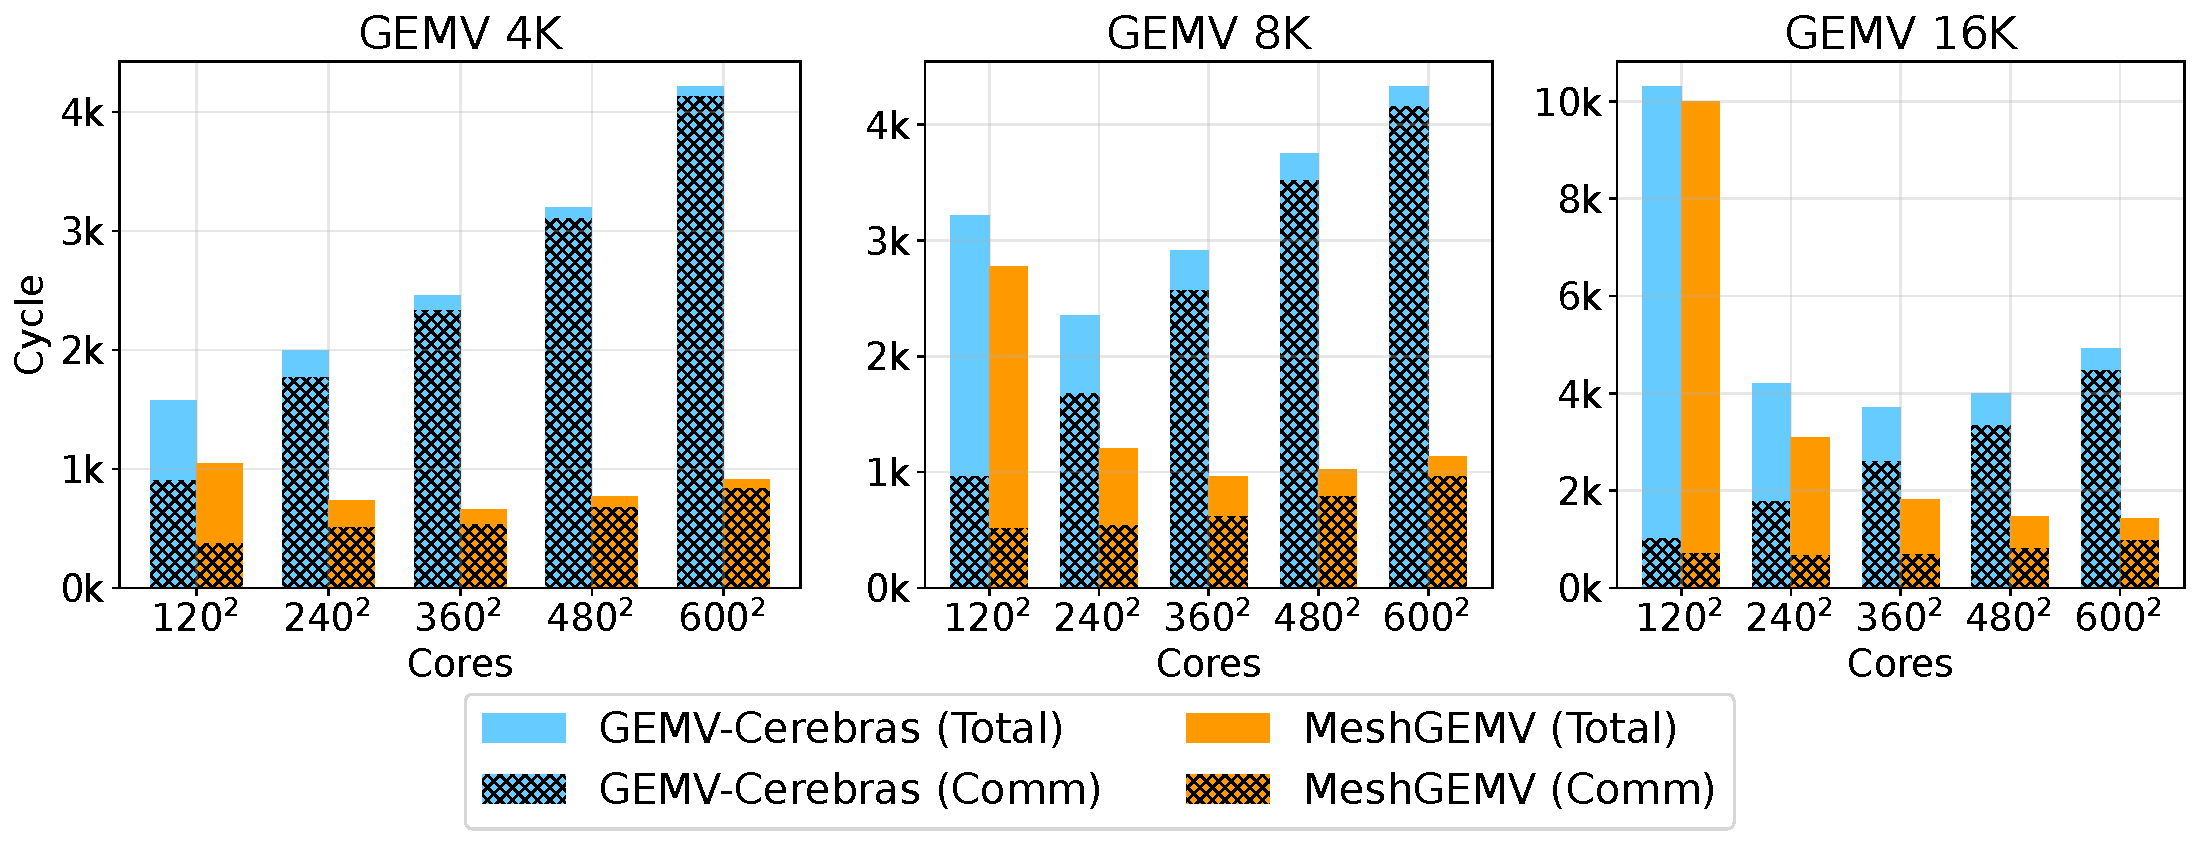
\includegraphics[width=1\linewidth]{imgs/gemv_micro_benchmark_combined.pdf}
    \caption{\gemv vs. GEMV-Cerebras}
    \vspace{-0.3cm}
    \label{fig:eval:meshgemv}
\end{figure}

\mypar{Communication latency bottleneck} Figure~\ref{fig:eval:meshgemv} shows that communication becomes the primary bottleneck for dist-GEMV computations on WSE-2, especially when the parallelism scale is large relative to the computation per core, where communication overhead can dominate 90\% of the total. However, \gemv significantly reduces communication overhead compared to the Cerebras baseline GEMV, achieving about 4.6$\times$ higher end-to-end performance. This is because large-scale dist-GEMV requires long-distance allreduce communication, and \gemv uses K-tree Allreduce to maximize parallelism in the allreduce process, minimizing communication and computation costs along the critical path.

\mypar{Scaling core count and matrix size} We also evaluate \gemv with larger matrix sizes. For GEMV 8K and 16K compared to 2K, the baseline shows a trend that the end-to-end overhead first decreases and then increases. The initial decrease comes from increased core count, where the higher aggregate compute power and bandwidth reduce computation and communication costs. However, as the core count grows, the communication latency of allreduce eventually overtakes computation and bandwidth as the dominant bottleneck. In contrast, \gemv's inflection point appears later, which means that for the same data size, \gemv's communication overhead grows much more slowly with increasing core count compared to the baseline, demonstrating better scalability. This enables more flexible on-chip mapping policies, such as using more cores to store additional LLM parameters to meet memory limitations (M) without introducing significant extra overhead.

\vspace{-0.3cm}
\subsection{Shift-based KV cache management}\label{sec:eval:kvcache}
\vspace{-0.2cm}

\begin{table}[t]
  \centering
  \resizebox{0.8
  \linewidth}{!}{
    \begin{tabular}{l|c|c}
    \hline
    Model & LLaMA3-8B & LLaMA2-13B \\
          \hline
    Concat-based (PagedAttention) & 382   & 16 \\
    \hline
    Shift-based (\sys) & 137548 & 6168 \\
    \hline
    \end{tabular}%
    }
  \caption{Maximum decode output length}
  \label{tab:eval:kvcache}%
\end{table}%


We also compare the shift-based KV cache management with the concat-based KV cache management in PagedAttention. We evaluate KV cache capacity on LLaMA3-8B and LLaMA2-13B using the same settings as the end-to-end inference evaluation in Section~\S\ref{sec:eval:e2e}. Table~\ref{tab:eval:kvcache} shows that \sys's shift-based KV cache management supports 360$\times$ and 385$\times$ more tokens than the concat-based method for LLaMA3-8B and LLaMA2-13B, respectively. This improvement results from balanced core utilization and the resolution of skewed data issues achieved by the shift-based approach.

\vspace{-0.2cm}
\subsection{Comparison with GPUs}\label{sec:eval:gpu}
\vspace{-0.2cm}

\begin{table}[t]
  \centering
  \resizebox{\linewidth}{!}{
    \begin{tabular}{c|ccc|ccc}
\hline
GEMV & \multicolumn{3}{c|}{[1,16K]$\times$[16K,16K]} & \multicolumn{3}{c}{[1,32K]$\times$[32K,32K]} \\ \hline
\multirow{2}{*}{\begin{tabular}[c]{@{}c@{}}TP in SGLang(A100)\\ Time (ms)\end{tabular}} & 1 GPU & 8 GPUs & 2$\times$8 GPUs & 1 GPU & 8 GPUs & 2$\times$8 GPUs \\ \cline{2-7} 
 & 0.336 & 0.253 & 0.340 & 1.231 & 0.341 & 0.339 \\ \hline
\begin{tabular}[c]{@{}c@{}}\gemv(WSE-2)\\ Time (ms)\end{tabular} &  & 0.0012 &  &  & 0.00203 &  \\ \hline
\begin{tabular}[c]{@{}c@{}}A100/WSE-2 Energy Ratio\end{tabular} & \textbf{7.47} & \textbf{44.97} & \textbf{120.88} & \textbf{16.17} & \textbf{35.83} & \textbf{71.25} \\ \hline
\end{tabular}%
    }
  \caption{Comparing \gemv(WSE-2) with TP in SGLang(A100) of GEMV latency and energy.}
  \vspace{-0.3cm}
  \label{tab:mv_gpu}%
\end{table}%

We compare \sys against the state-of-the-art LLM inference system on GPUs using Cerebras WSE-2 and NVIDIA A100. To compare against the H100 fairly, we would need access to the WSE-3, which is a 5nm manufacturer but unavailable to us.

\mypar{GEMV} We compared \gemv with the GEMV parallelization strategy that follows SGLang's \cite{sglang} multi-GPU tensor parallelism, while the computation on each GPU is accelerated using the cuBLAS library. Shown by Table~\ref{tab:mv_gpu}, compared to a single A100 GPU, \gemv outperforms by 280-606$\times$ with different matrix sizes, showcasing the advantages of providing substantial memory bandwidth through wafer-scale devices. This also translates to 7.5-16$\times$ greater energy efficiency, reflecting the benefits of wafer-based connections (connecting on-chip memory) over PCB-based ones (connecting off-chip HBM) in GPUs.

Distributed GEMV on multi-GPUs shows limited scalability: a single A100 yields the highest energy efficiency per FLOP, and performance improves only 1.32$\times$ from one to eight GPUs, then degrades at sixteen. This inefficiency stems from memory intensity and communication overhead over NVLink and IB. In contrast, \gemv exploits WSE-2's low-latency NoC to scale across hundreds of thousands of cores, achieving 166-210$\times$ higher performance and 45-70$\times$ better energy efficiency at peak compared to the best GPU cluster results. Moreover, GEMV exhibits similar performance for 16K and 32K tasks on two machines with 16 GPUs, mainly because communication overhead dominates the computation in distributed GEMV across two nodes.

Despite these advantages, \gemv does not achieve the theoretical 7,000$\times$ improvement. Profiling identifies three contributing factors: (i)~WSE-2 cores, still in their second generation, cannot fully overlap memory access and computation; (ii)~edge cores are underutilized; and (iii)~NoC long-range communication overhead persists, despite \gemv mitigating it effectively. We anticipate these gaps will continue to narrow as wafer-scale accelerators mature.

\begin{table}[t]
  \centering
  \resizebox{\linewidth}{!}{
    \begin{tabular}{c|ccc|cc}
\hline
Prefill (4K CTX) & \multicolumn{3}{c|}{LLaMA3-8B} & \multicolumn{2}{c}{LLaMA2-13B} \\ \hline
\multirow{2}{*}{\begin{tabular}[c]{@{}c@{}}SGLang(A100) TPR\end{tabular}} & 1 GPU & 8 GPUs & 2$\times$8 GPUs & 1 GPU & 8 GPUs \\ \cline{2-6} 
 & 13988 & 17361 & 13994 & 7805 & 12287 \\ \hline
\begin{tabular}[c]{@{}c@{}}\sys WSE-2 TPR\end{tabular} &  & 27686 &  & \multicolumn{2}{c}{17498} \\ \hline
A100/WSE-2 Energy Ratio & \textbf{0.05} & \textbf{0.34} & \textbf{0.84} & \textbf{0.06} & \textbf{0.30} \\ \hline
\end{tabular}%
    }
  \caption{Comparing \sys(WSE-2) with SGLang(A100) in prefill throughput and energy.}
  \vspace{-0.3cm}
  \label{tab:llmoc_gpu_prefill}%
\end{table}%

\begin{table}[t]
  \centering
  \resizebox{\linewidth}{!}{
    \begin{tabular}{c|ccc|cc}
\hline
Decode (4K CTX) & \multicolumn{3}{c|}{LLaMA3-8B} & \multicolumn{2}{c}{LLaMA2-13B} \\ \hline
\multirow{2}{*}{\begin{tabular}[c]{@{}c@{}}SGLang(A100) TPR\end{tabular}} & 1 GPU & 8 GPUs & 2$\times$8 GPUs & 1 GPU & 8 GPUs \\ \cline{2-6} 
 & 78 & 260 & 164 & 48 & 175 \\ \hline
\begin{tabular}[c]{@{}c@{}}\sys WSE-2 TPR\end{tabular} &  & 2700 &  & \multicolumn{2}{c}{2039} \\ \hline
A100/WSE-2 Energy Ratio & \textbf{0.92} & \textbf{2.22} & \textbf{7.02} & \textbf{1.13} & \textbf{2.49} \\ \hline
\end{tabular}%
    }
  \caption{Comparing \sys(WSE-2) with SGLang(A100) in decode throughput and energy.}
  \vspace{-0.3cm}
  \label{tab:llmoc_gpu_decode}%
\end{table}%

\mypar{LLM inference} The maximum TPR achievable on GPU clusters is significantly lower than on WSE-2. We compare \sys with SGLang on an A100 multi-GPUs cluster and find that \sys delivers a 6-20$\times$ higher TPR across a range of input/output lengths and model sizes from 8B to 72B, with the gap widening for longer outputs and larger models (Table~\ref{tab:e2e_table}). As shown in Tables~\ref{tab:llmoc_gpu_prefill} and \ref{tab:llmoc_gpu_decode}, scaling SGLang from 1 to 8 GPUs yields only 1.2-1.6$\times$ prefill and 3.3-3.6$\times$ decode speedups, far below ideal linear scaling. Performance further degrades when scaling to 16 GPUs, due to inter-node communication bottlenecks. As a result, peak TPR for dense models is typically reached within a single 8-GPU node, where \sys still outperforms SGLang up to 20$\times$. For use cases demanding high per-request throughput, wafer-scale accelerators are substantially more capable than conventional xPU-based systems.

In terms of energy efficiency, though a WSE-2 chip has ~47$\times$ the area and ~37$\times$ the power and cost of an A100, \sys still achieves a 2-2.5$\times$ energy efficiency advantage at SGLang's optimal multi-GPU result, owing to GPUs' nonlinear scaling on decode. This advantage is especially valuable for long-output scenarios like test-time scaling, where serving cost is critical. However, compared to GEMV, \sys's decode energy efficiency advantage is reduced due to: (i) limited local SRAM (48KB) on WSE-2 cores, which hinders efficient tensor parallelism and necessitates pipeline parallelism, causing up to 5$\times$ underutilization; and (ii) GPU-optimized LLaMA models with narrow layers that constrain layer placement and worsen utilization on WSE-2.

